\section{Le logiciel}
L’objectif du logiciel est d’éditer des devis et factures et de proposer une gestion des clients :
le client possède un ou plusieurs projets auxquels sont associés un ou plusieurs devis et/ou factures.
Ainsi, l’architecture logicielle comporte une base de données de type SQLite pour la gestion des
clients, de ses projets, des devis et factures associés. Nous utilisons un patron de conception MVC,
avec un modèle qui correspond aux objets métiers Client, Projet, Factures, Devis, Prestations. Ces
objets sont instanciés par les classes associées à la base de données qui réalisent ces tâches. Enfin,
nous générerons les devis et factures en LaTeX ou en PDF.

\subsection{Fenêtre principale}
\begin{figure}[H]
	\centering
	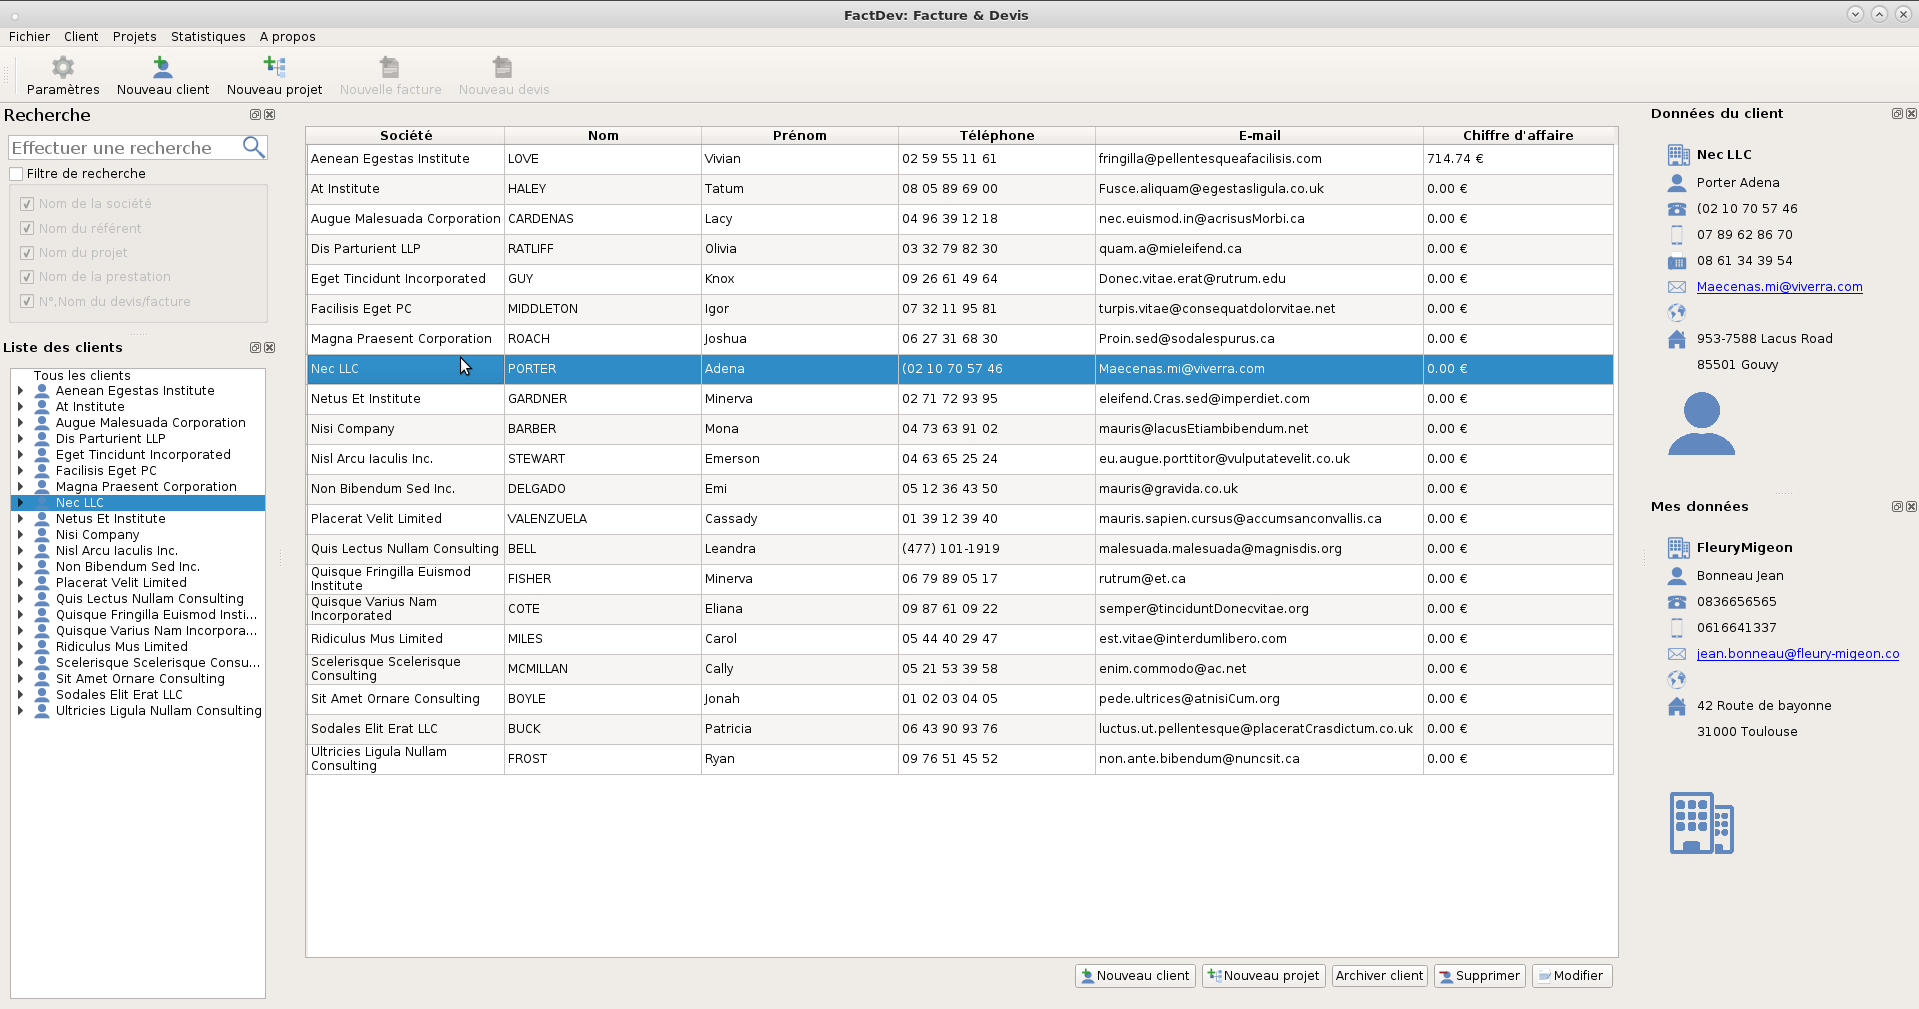
\includegraphics[width=17cm]{screens/ihmClients.png}
	\caption{Fenêtre principale du logiciel \FactDev}
	\label{fig:principal_window}
\end{figure}

Voici la fenêtre principale qui s'affiche au lancement du logiciel. Elle permet d'avoir un accès rapide aux clients, qui sont l'élément principal du logiciel.

\subsubsection{Tableau des clients}
\begin{figure}[H]
	\centering
	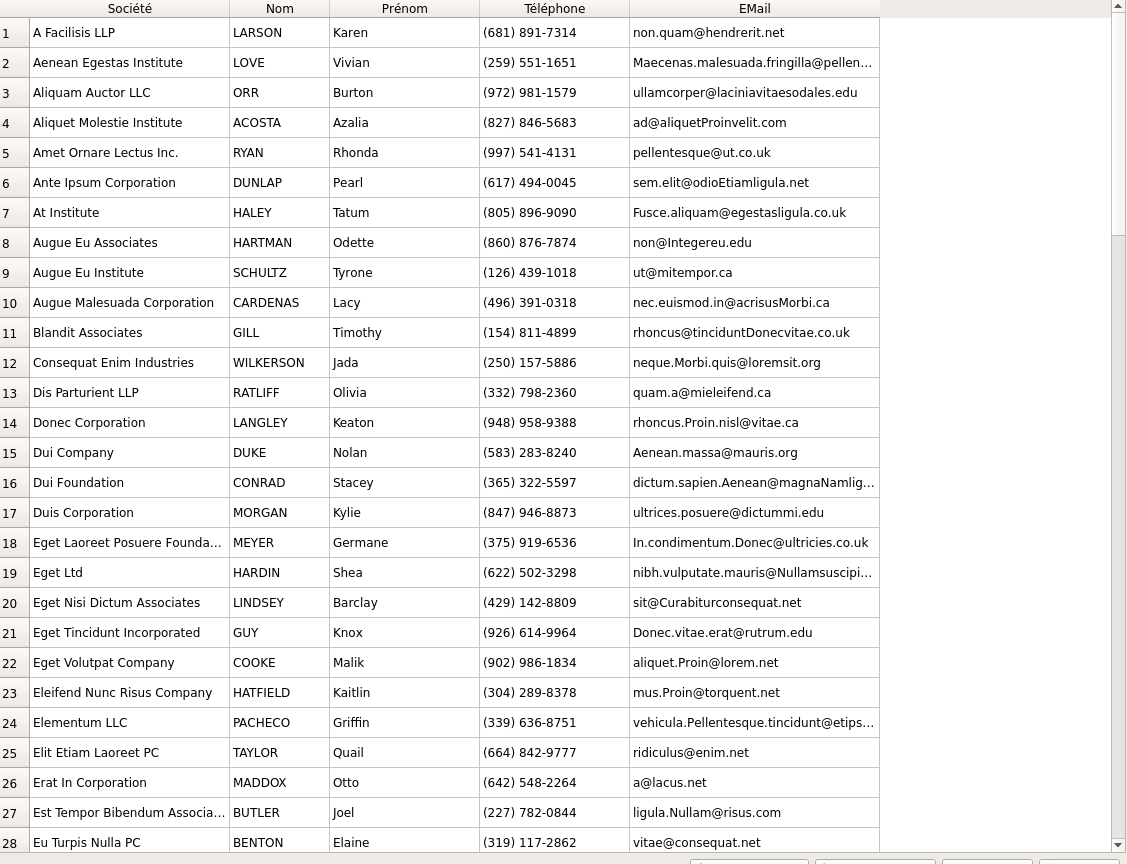
\includegraphics[width=15cm]{screens/clients.png}
	\caption{Le tableau des clients}
	\label{fig:customers_table}
\end{figure}

Le tableau des clients contient uniquement les informations permettant de facilement les identifier à
savoir, le nom de la société, le nom, prénom, le numéro de téléphone et l’adresse e-mail. La sélection
dans le tableau de l’un des clients permet, via le panneau du client, d’obtenir les informations
détaillées sur celui-ci (cf \ref{fig:customer_data}). Trois possibilités sont données à partir de ce tableau: 
\begin{description}
	\item[L'ajout] de clients
	\item[La suppression] de clients (sous certaines conditions)
	\item[L'archivage] de clients
\end{description}

\subsubsection{Arbre des clients}
\begin{figure}[H]
	\centering
	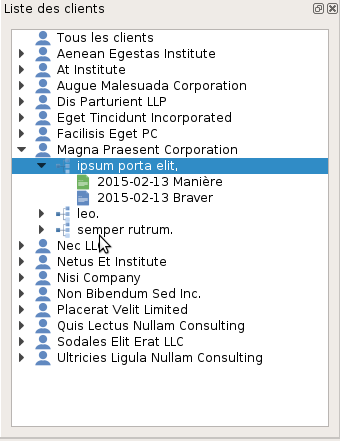
\includegraphics[width=8cm]{screens/dockHierarchique.png}
	\caption{L'arbre des clients}
	\label{fig:customers_tree}
\end{figure}
Ce panneau hiérarchique, initialement situé en bas à gauche de la fenêtre principale, comporte une
vue hiérarchique de l’ensemble des clients et des projets associés à chacun de ces clients. Des devis
et des factures sont associés à chacun de ces projets.

\subsubsection{Recherche de Clients}
\begin{figure}[H]
	\centering
	
\includegraphics[width=8cm]{screens/dockRecherche.png}
	\caption{Le panneau de recherche des clients}
	\label{fig:customers_search}
\end{figure}
Le panneau de recherche, situé en haut à gauche de la fenêtre principale, permet d’effectuer une recherche selon le nom de
la société, le nom du client, du référent, du projet, d’une prestation ou le numéro et le nom d’un
devis ou d’une facture si la case filtre de recherche est cochée. Cela permet de retrouver rapidement
et facilement un client, un projet, un devis, une facture ou même une prestation.

\subsubsection{Données du Client}
\begin{figure}[H]
	\centering
	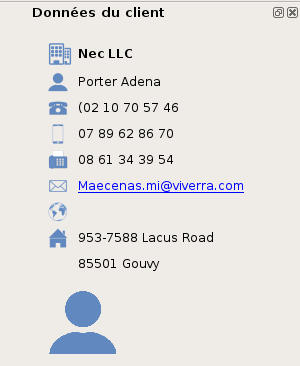
\includegraphics[width=8cm]{screens/dockDroite.png}
	\caption{Les données du client sélectionné}
	\label{fig:customer_data}
\end{figure}
Le panneau initialement situé en haut à droite de la fenêtre principale contient les informations du client ou du référent
sélectionné dans le tableau des clients (cf \ref{fig:customers_table}).

\subsubsection{Données de l'utilisateur}
\begin{figure}[H]
	\centering
	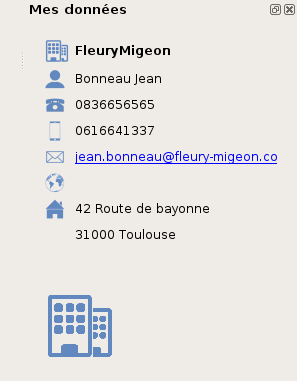
\includegraphics[width=8cm]{screens/dockUtilisateur.png}
	\caption{Les données de l'utilisateur du logiciel}
	\label{fig:user_data}
\end{figure}
Le panneau initialement situé en bas à droite contient les informations de l’utilisateur qui ont préalablement été rentrées lors d'un lancement antérieur.

\subsection{Factures/Devis}
\begin{figure}[H]
	\centering
	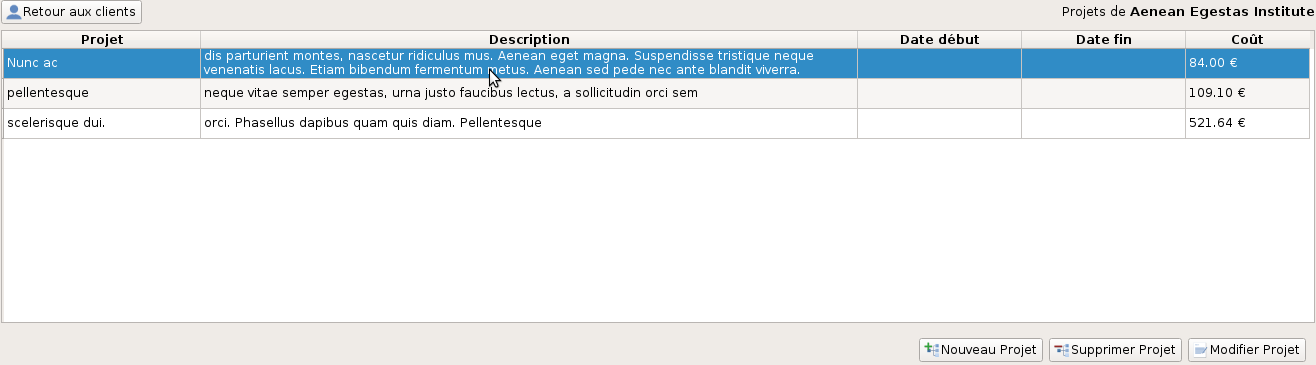
\includegraphics[width=17cm]{screens/projets.png}
	\caption{L'édition d'une facture}
	\label{fig:edit_fact}
\end{figure}
L'ajout d'une facture ou d'un devis se déroule de la même façon que l'édition d'une facture ou d'un devis. Le devis et la facture ont en effet le même comportement.

\subsubsection{Description}
\begin{figure}[H]
	\centering
	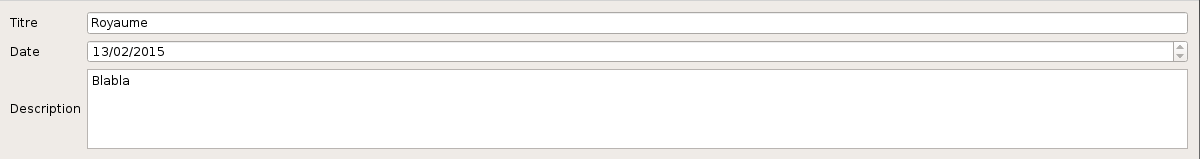
\includegraphics[width=17cm]{screens/description.png}
	\caption{L'édition d'une facture}
	\label{fig:description_fact}
\end{figure}
Une facture possède un titre à afficher, une date et une description. Si le titre et la description de la facture sont éditables, la date est définie par défaut à la date de création de la facture et n'est pas modifiable.

\subsubsection{Liste des projets}
\begin{figure}[H]
	\centering
	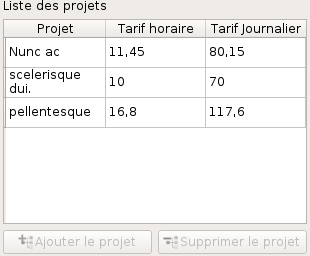
\includegraphics[width=8cm]{screens/listeProjets.png}
	\caption{La liste des projets concernés par la facture}
	\label{fig:project_list_bill}
\end{figure}
Une facture possède une liste de projets (ceux du client concerné) avec un tarif journalier et un tarif horaire qui sont tout les deux modifiables. En sachant que la modification de l'un entraînera bien sûr la modification de l'autre et vice-versa.

\subsubsection{Liste des prestations}
\begin{figure}[H]
	\centering
	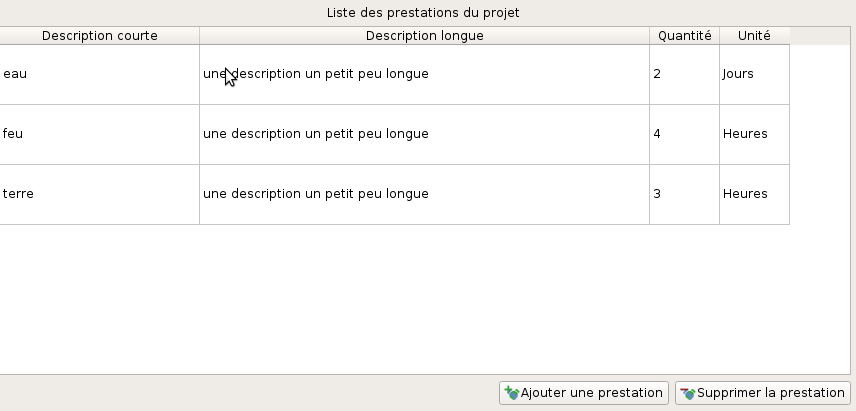
\includegraphics[width=12cm]{screens/listePrestations.png}
	\caption{La liste des prestations}
	\label{fig:prestation_list}
\end{figure}
Chaque prestation est définie par:
\begin{description}
	\item[une description courte]
	\item[une description longue]
	\item[une quantité de travail]
	\item[l'unité de cette quantité]
\end{description}
Chacun des champs sont éditables en sachant que la modification du champ <<quantité>> ou <<unité>> aura une influence sur le calcul des coûts.

\subsubsection{Calcul des coûts}
\begin{figure}[H]
	\centering
	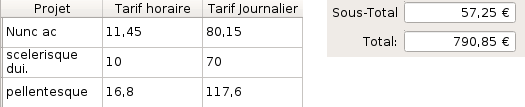
\includegraphics[width=10cm]{screens/calculCouts.png}
	\caption{Le calcul des coûts est automatique.}
	\label{fig:compute_costs}
\end{figure}
Tout les prix
affichés, que cela soit le sous-total (total d’un projet) ou le total de tous les projets, tous sont
calculés automatiquement en fonction du tarif horaire et journalier défini pour le projet et de la
quantité de temps définie pour une prestation.

\subsection{Génération}
\begin{figure}[H]
	\centering
	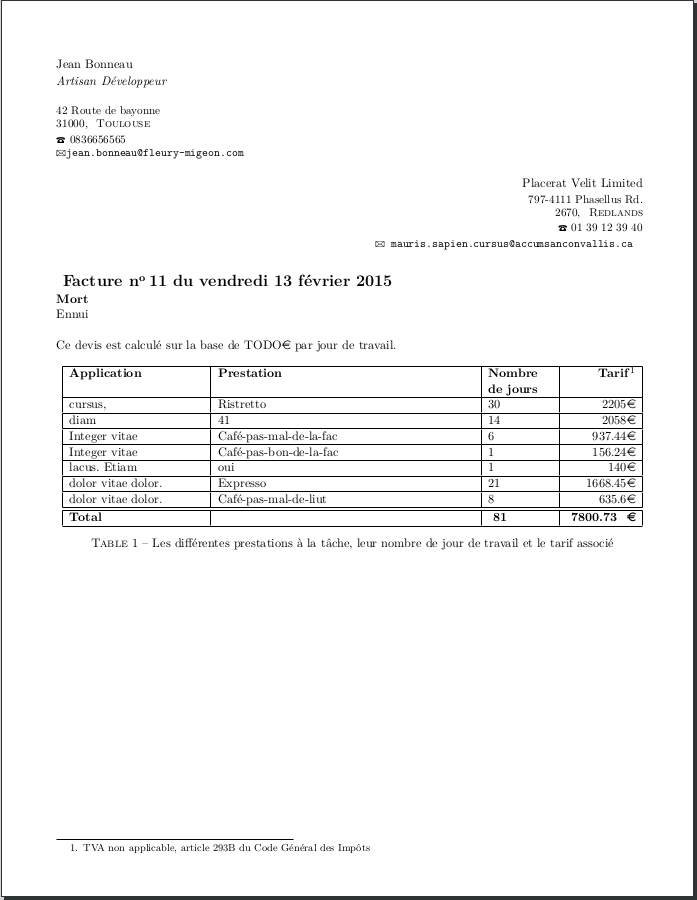
\includegraphics[width=17cm]{screens/genererPDF.png}
	\caption{PDF généré à partir d'une facture.}
	\label{fig:bill_pdf}
\end{figure}
Les factures et les devis présents en base de données ont tous la possibilité d'être généré en PDF.